\documentclass[12pt,A4]{article}

\usepackage{myStyle}
\usepackage{tikz}         % package to draw DAGs
\usepackage{subcaption}   % add spacing between DAGs

\usetikzlibrary{positioning, calc, shapes.geometric, shapes.multipart,
shapes, arrows.meta, arrows,
decorations.markings, external, trees}

\begin{document}

%Create custom arrow style:
\tikzstyle{Arrow} = [
	thick,
	decoration={
	markings,
	mark=at position 1 with {
	\arrow[thick]{latex}
		}
	},
	shorten >= 3pt, preaction = {decorate}
]

\newpage

% Time-varying confounding
%\begin{tikzpicture}[
%    >={Stealth[round]}, % Stealth arrows
%    shorten >=1pt,
%    auto,
%    node distance=2.5cm and 3cm,
%    thick
%]
%% Define nodes
%\node (Z) {Random assignment};  % Instrumental Variable
%\node (A0) [right of=Z, xshift=2cm] {$A_0$};  % First Treatment
%\node (A1) [right of=A0, xshift=2cm] {$A_1$};  % Second Treatment
%\node (Y)  [right of=A1, xshift=2cm] {$Y_2$};  % Outcome
%\node (L0) [above of=A0, yshift=1cm] {$L_0$};  % Confounder at Time 0
%\node (L1) [above of=A1, yshift=1cm] {$L_1$};  % Confounder at Time 1
%% Draw edges (arrows)
%\draw[->] (Z) -- (A0);  % Z to A0
%\draw[->] (A0) -- (A1);  % A0 to A1
%\draw[->] (A1) -- (Y);   % A1 to Y
%\draw[->] (L0) -- (A0);  % L0 to A0 (confounding A0)
%\draw[->] (L0) -- (A1);  % L0 to A1 (time-varying confounding)
%\draw[->] (L1) -- (A1);  % L1 to A1 (confounding A1)
%\draw[->] (L1) -- (Y);   % L1 to Y (confounding Y)
%\draw[->] (A0) -- (L1);  % A0 to L1 (time-varying effect)
%\draw[->] (L0) -- (L1);  % L0 to L1 (time-varying confounding)
%\end{tikzpicture}


% Time-varying confounding
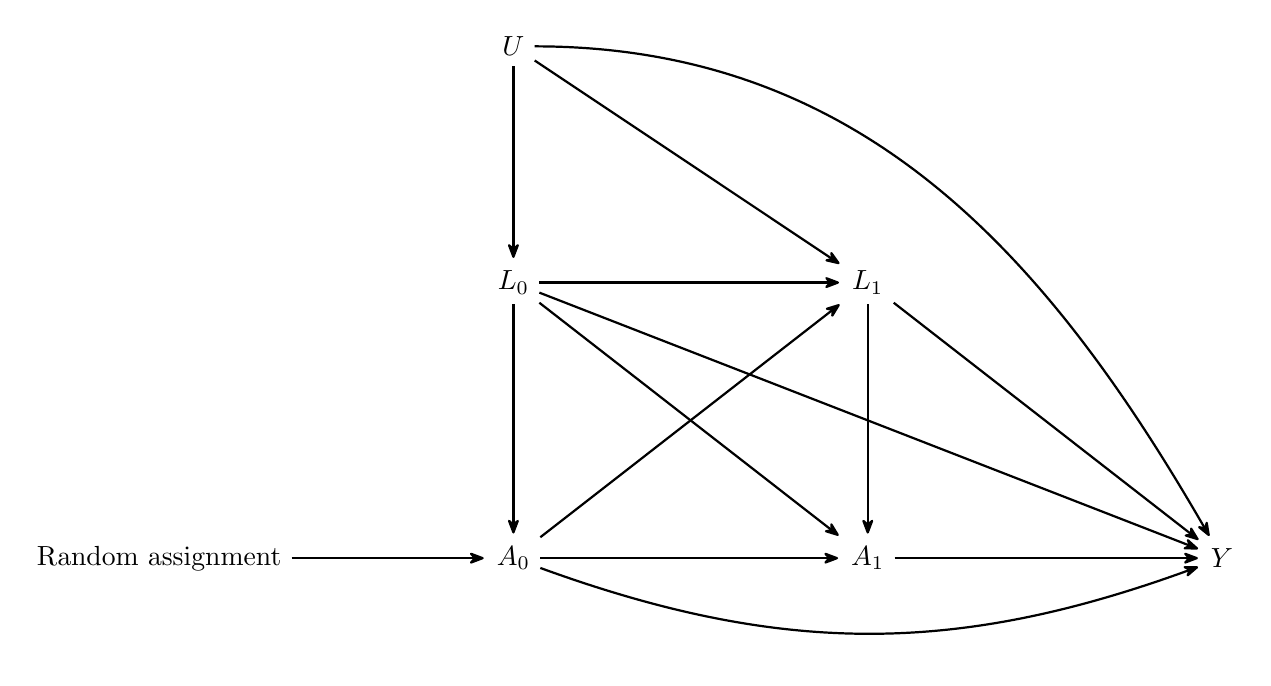
\begin{tikzpicture}[
    >={Stealth[round]},
    shorten >=1pt,
    auto,
    node distance=2.5cm and 3cm,
    thick
]

% Define nodes
\node (Z) {Random assignment};
\node (A0) [right of=Z, xshift=2cm] {$A_0$};
\node (A1) [right of=A0, xshift=2cm] {$A_1$};
\node (Y)  [right of=A1, xshift=2cm] {$Y$};
\node (L0) [above of=A0, yshift=1cm] {$L_0$};
\node (L1) [above of=A1, yshift=1cm] {$L_1$};

% U closer to L0
\node (U)  [above of=L0, yshift=0.5cm] {$U$};

% Main edges
\draw[->] (Z) -- (A0);
\draw[->] (A0) -- (A1);
\draw[->] (A1) -- (Y);
\draw[->] (L0) -- (A0);
\draw[->] (L0) -- (A1);
\draw[->] (L1) -- (A1);
\draw[->] (L1) -- (Y);
\draw[->] (A0) -- (L1);
\draw[->] (L0) -- (L1);

% Additional arrows
\draw[->] (L0) -- (Y);                         % Straight L0 -> Y2
\draw[->, out=-20, in=-160] (A0) to (Y);       % Reduced curvature A0 -> Y2

% U edges
\draw[->] (U) -- (L0);
\draw[->] (U) -- (L1);
\draw[->, out=0, in=120] (U) to (Y);

\end{tikzpicture}


\par\bigskip
\par\bigskip

\textbf{Fig 1.} Causal directed acyclic graph demonstrating the potential for confounding after random assignment in a randomized clinical trial.
Nodes are $A_0$ and $A_1$: treatment at baseline time 0 and follow-up time 1, $L_0$ and $L_1$: confounders of adherence and loss to follow-up at time 0 and time 1, $U$: unmeasured confounders, and $Y$: outcome. 
%Arrows show directions of causal effects, and indicate how present treatment and confounders ($A_0$, $L_0$) affect future treatment and confounders ($A_1$, $L_1$). 
%Note that $L_1$ is a common cause (\textit{confounder}) of $A_1$ and $Y_2$ and needs to be adjusted for, but $L_1$ is also a common effect (\textit{collider}) of $L_0$ and $A_0$ and adjusting for $L_1$ will introduce collider stratification bias.
%Conventional methods that statistically adjust for confounders cannot be applied to minimize post-randomization confounding. Generalized methods (g-methods) are needed to minimize time-varying confounding by balancing the distribution of confounders between groups using weighting procedures. This effectively removes arrows into and out of confounders, allowing an unbiased effect of treatment to be estimated. 

\end{document}
